%\documentclass[11pt,professionalfonts,hyperref={pdftex,pdfpagemode=none,pdfstartview=FitH}]{beamer}
%\usepackage{times}
\documentclass[11pt,professionalfonts]{beamer}
\usefonttheme{serif}
\usepackage{presentation_packages}
\usepackage[version=3]{mhchem}
\DeclareSIUnit\year{yr}
\newcommand{\hilight}[1]{\colorbox{green}{#1}}

\definecolor{mygray}{gray}{0.9}
\definecolor{RoyalBlue}{rgb}{0.25,0.41,0.88}
\def\Emph{\textcolor{RoyalBlue}}

\definecolor{tmp}{rgb}{0.804,0.941,1.0}
\setbeamercolor{numerical}{fg=black,bg=tmp}
\setbeamercolor{exact}{fg=black,bg=red}

\mode<presentation> 
{
  \usetheme{Warsaw}
  \usefonttheme{serif}
  \setbeamercovered{transparent}
}

\setbeamertemplate{footline}%{split theme}
{%
  \leavevmode%
  \hbox{\begin{beamercolorbox}[wd=.5\paperwidth,ht=2.5ex,dp=1.125ex,leftskip=.3cm,rightskip=.3cm plus1fill]{author in head/foot}%
    \usebeamerfont{author in head/foot}\insertshorttitle
  \end{beamercolorbox}%
  \begin{beamercolorbox}[wd=.5\paperwidth,ht=2.5ex,dp=1.125ex,leftskip=.3cm,rightskip=.3cm]{title in head/foot}
%    \usebeamerfont{title in head/foot}\mypaper\hfill \insertframenumber/\inserttotalframenumber
    \usebeamerfont{title in head/foot}\hfill \insertframenumber/\inserttotalframenumber
  \end{beamercolorbox}}%
  \vskip0pt%
} \setbeamercolor{box}{fg=black,bg=yellow}


\title[Autonomous Landing]{\large\textbf Geometric Control for Autonomous Landing on Asteroid Itokawa using Visual Localization}

\author{\vspace*{-0.3cm}}
   
\institute{
	\footnotesize
	{\normalsize\bf{Shankar Kulumani, Kuya Takami \\ Taeyoung Lee}}\\
	\vspace*{0.2cm}
  	\textbf{Department of Mechanical \& Aerospace Engineering}\\ \vspace*{0.5cm}
 	\begin{figure} %figure%
       	
\includegraphics[width=0.75\textwidth]{gw_txh_2cs_pos}
  	\end{figure}
}
\date{\today}

\begin{document}
%=======================================================%

\setcounter{framenumber}{-1}
\begin{frame} %-----------------------------%
  \titlepage
\end{frame}   %-----------------------------%

\section*{}
\subsection*{Introduction}  
\begin{frame}{Asteroid Missions}
\begin{itemize}
    \item Science - insight into the early formation of the solar system
    \item Mining - vast quantities of useful materials
    \item Impact - high risk from hazardous near-Earth asteroids
\end{itemize}    

\begin{center}
    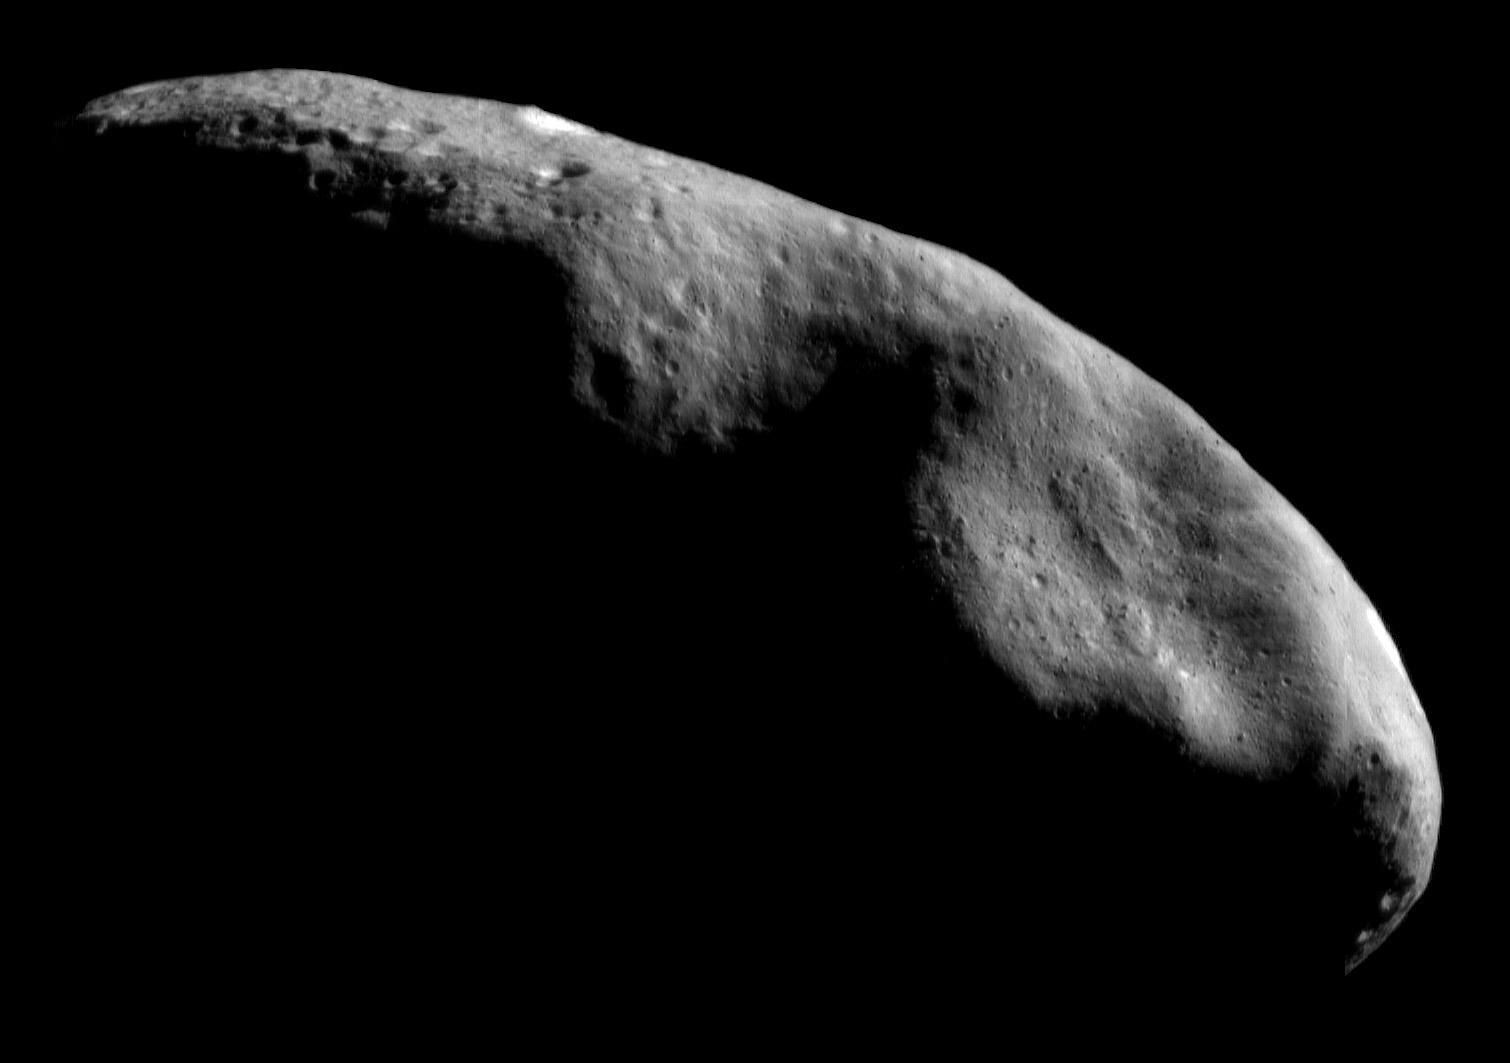
\includegraphics[height=0.35\textheight]{figures/near_mos_20001203_full.jpg}
    \hfill
    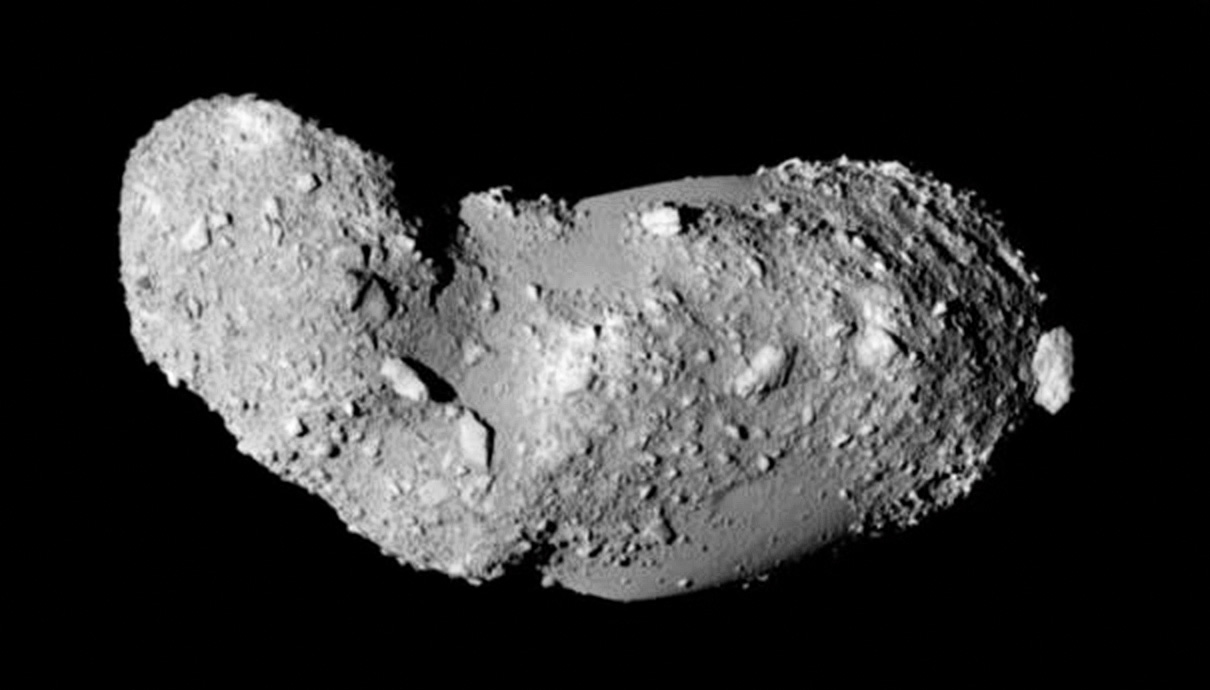
\includegraphics[height=0.35\textheight]{figures/Itokawa8_hayabusa_1210.jpg}
\end{center}
\end{frame}

\begin{frame}{Asteroid Mining}
    \begin{itemize}
      \item Useful materials can be extracted from asteroids to support:
      \begin{itemize}
          \item Propulsion, construction, life support, agriculture, and precious/strategic metals
      \end{itemize}
        \pause
      \item Commercialization of near-Earth asteroids is feasible
    \end{itemize}


\begin{center}
\small
    \begin{tabular}{|l|r|r|}
        \hline 
        Element & Price (\SI{}[\$\,]{\per\kilo\gram}) & Sales (\SI{}[\$\,]{M\per\year}) \\
        \hline \hline 
        Phosphorous (P) & \num{0.08}  & \num{2167} \\
        Gallium (Ga) & \num{300.00}  & \num{1544} \\
        Germanium (Ge) & \num{745.00} & \num{6145} \\
        \hline \hline 
        Platinum (Pt) & \num{12394.00} & \num{1705} \\
        Gold (Au) & \num{12346.00} & \num{49} \\
        Osmium (Os) & \num{12860.00} & \num{307} \\
        \hline
    \end{tabular}
\end{center}

\end{frame}

\section*{}
\subsection*{Motivation}  

\begin{frame}{Asteroid Landing}
    \begin{itemize}
        \item Long history of asteroid/planetary missions
            \begin{itemize}
                \item NEAR, Hayabusa, OSIRIS-REX, Rosetta
            \end{itemize}
            \pause
        \item Asteroid landing is particularly challenging:
            \begin{itemize}
                \item<3-> Challenging dynamics - low gravity and spinning
                \item<4-> Poor model - ground based observation of dim bodies
                \item<5-> Attitude coupling - pertubations are large 
            \end{itemize}
    \end{itemize}
    \begin{center}
        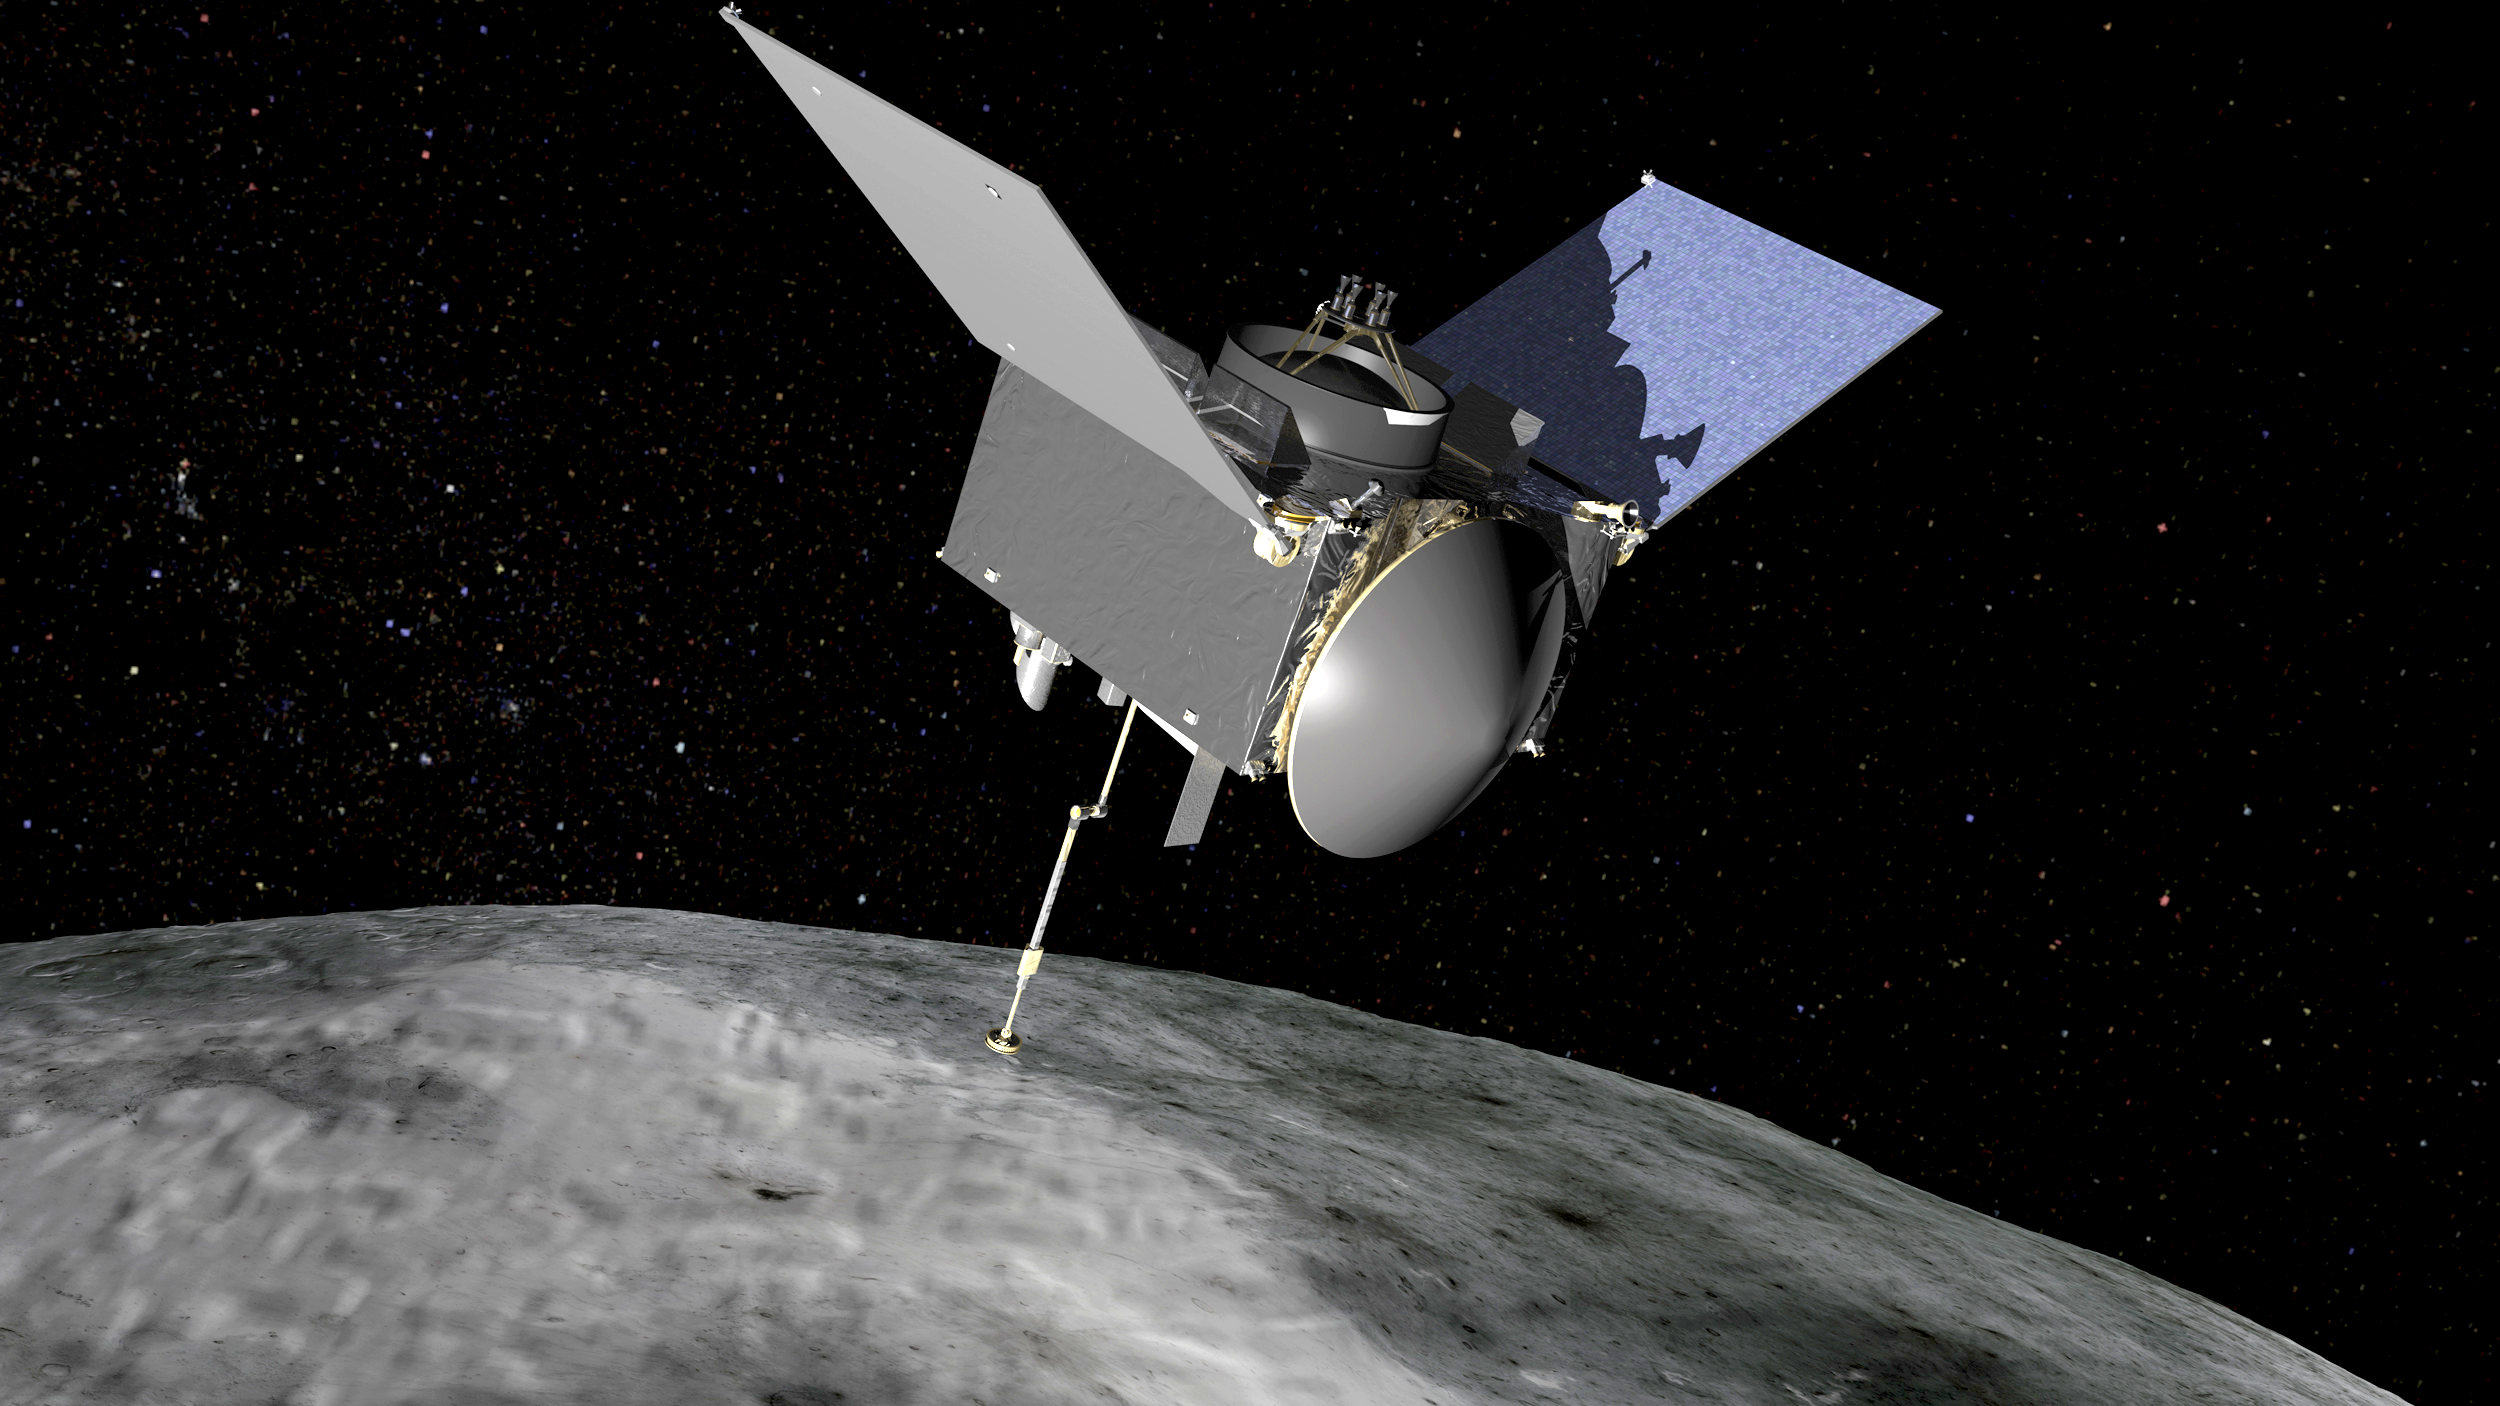
\includegraphics[width=0.6\textwidth,height=0.4\textheight,keepaspectratio]{figures/osiris_rex.png}~
        \includegraphics[width=0.6\textwidth,height=0.4\textheight,keepaspectratio]{figures/Rosetta_Philae_Artist_Impression_Close_4k.jpg}
    \end{center} 
\end{frame}

\begin{frame}{Problem Statement}
    \begin{enumerate}
        \item Develop copuled equations of motion for a spacecraft
        \item EOMs on \( \SE \) to derive landing control law
            \begin{itemize}
                \item \( \SE \) - special euclidean group describes the general motion of rigid bodies
            \end{itemize}
        \item Implement monocular localization to provide state estimates
        \item Alleviates many of the issues of past approaches:
            \pause
            \begin{itemize}
                \item Explicitly consider rotational dynamics
                \item Geometric control defined directly on \( \SE \)
                \item Onboard state measurements for ``autonomy''
            \end{itemize}
    \end{enumerate}
\end{frame}
\section*{}
\subsection*{Mathematical Background}

\begin{frame}{Attitude Parameterizations}
	\begin{itemize}
		\item Euler Angles
		\begin{itemize}
			\item Minimal representation used for small attitude changes.
			\item Singularities exist for large angle slews: requires switching between 24 sequences
			\item Complicated trigonometric functions
		\end{itemize}
		\pause
		\item Quaternion 
		\begin{itemize}
			\item No singularities
			\item Two anti-podal quaternions for the same attitude
			\item Unwinding behavior for control systems
		\end{itemize}
		\pause
		\item Geometric control
		\begin{itemize}
			\item Globally and uniquely characterize attitude: \( R \in \SO \)
			\item Controller is globally valid for large angle maneuvers
		\end{itemize}
	\end{itemize}
	
    \end{frame}
\begin{frame}{Gravitational Modeling} %-----------------------------%

\begin{itemize}
  \item Asteroids are extended bodies not point masses
  \pause
  \item Spherical Harmonic - only valid outside of circumscribing sphere
    {
    \small
    \begin{align*}
      U(\vecbf{r} ) = \frac{\mu}{r} \sum_{n=0}^\infty \sum_{m=0}^\infty \parenth{\frac{R}{r}}^nP_{n,m}(\sin \phi) \braces{ C_{nm} \cos(m \lambda) + S_{nm} \sin(m \lambda)} 
    \end{align*}
    }
    \pause
  \item Infinite series is an approximation and adds complexity
    \begin{itemize}
        \item Model switching at circumscribing sphere
        \item Coefficient matching used to ensure continuity 
    \end{itemize}
\end{itemize}

\note[itemize]{
  \item Models require detailed data from orbit about asteroid (OD process determines gravity field)
  \item Simplified models (triaxial ellipsoid allows analytical insight)
  \item Previous work fails to consider coupled dyanmics
  }

\end{frame}   %-----------------------------%


\begin{frame}{Polyhedron Gravitation Model}

\begin{itemize}
    \item Potential is a function of only the shape model
    \item Globally valid, closed-form expression of potential
    \item Exact potential assumes a constant density 
    \item Accuracy solely dependent on shape model
\end{itemize}
\only<2>{
\begin{align*}\label{eq:potential}
    U(\vecbf{r}) &= \frac{1}{2} G \sigma \sum_{e \in \text{edges}} \vecbf{r}_e \cdot \vecbf{E}_e \cdot \vecbf{r}_e \cdot L_e - \frac{1}{2}G \sigma \sum_{f \in \text{faces}} \vecbf{r}_f \cdot \vecbf{F}_f \cdot \vecbf{r}_f \cdot \omega_f 
\end{align*}
}

\end{frame}

\begin{frame}{Kinematics of Dumbbell}
    \begin{itemize}
        \item Dynamics derived on \SE, Special Euclidean group
        \item Rigid dumbbell model - captures attitude coupling
        \pause
        \begin{itemize}
            \item \( \vecbf{x} \in \R^3 \) - inertial position of COM
            \item \( R \in \SO\) - transforms from body to inertial frame
            \item \( \vecbf{\Omega} \in \R^3 \) - the angular velocity of the spacecraft 
            \item \( R_A \in \SO \) - transforms from asteroid to inertial frame
        \end{itemize}    
        \pause
    \item Simple model which captures dynamic coupling  
        \begin{itemize}
            \item Models the mass distribution of spacecraft 
        \end{itemize}
        \pause
    \item Preserves the geometric properties of configuration space
    \item Attitude and Translational motion is directly coupled
\end{itemize}

\end{frame}

\begin{frame}{Equations of Motion}

    \begin{itemize}
        \item Polyhedron potential in translational and rotational dynamics
        \begin{align*}
            \dot{\vb{x}} &= \vb{v}, \\
            \parenth{m_1 + m_2} \dot{\vecbf{v}} &= m_1 R_A \deriv{U}{\vecbf{z}_1} + m_2 R_A \deriv{U}{\vecbf{z}_2} + \vecbf{u}_f, \\
            \dot{R} &= R S(\vb{\Omega}) , \\
            J \dot{\vecbf{\Omega}} + \vecbf{\Omega} \times J \vecbf{\Omega} &= \vecbf{M}_1 + \vecbf{M}_2 + \vecbf{u}_m. 
        \end{align*}
    \item Moment on dumbbell
        \begin{align*}
            \vecbf{M}_i = m_i \parenth{S(R_A^T \vb{\rho}_i) R^T \deriv{U}{\vb{z}_i}}.
        \end{align*}
    \end{itemize}
\end{frame}

\section*{}
\subsection*{Geometric Control}
\begin{frame}{Nonlinear Control}
    \begin{itemize}
        \item Geometric control used to track a desired trajectory
        \item Developed directly on the nonlinear manifold
            \begin{itemize}
                \item Avoids chattering issues of sliding mode control
                \item Incorporates attitude dynamics
                \item Asymptotic trajectory tracking stability
            \end{itemize}
    \end{itemize}

\pause
\begin{align*}
    \vb{u}_m &= - k_R e_R - k_\Omega e_\Omega + \Omega \times J \Omega - J \parenth{\hat{\Omega} R^T R_d \Omega_d - R^T R_d \dot{\Omega}_d}  \\
             &- \vb{M}_1 - \vb{M_2} , \\
    \vb{u}_f &= - k_x e_x  - k_v e_v + ( m_1  + m_2 ) \ddot{x}_d - \vb{F}_1 - \vb{F}_2 
\end{align*}
\end{frame}



\section*{}
\subsection*{Numerical Simulation}

\begin{frame}{Landing Trajectory - Attitude}
    \begin{itemize}
        \item Goal: transition from  orbit about Itokawa to vertical descent
        \item Attitude controlled to point camera at surface
            \begin{itemize}
                \item \( \vb{b}_1 \) - body axis points at surface
                \item \( \vb{b}_3 \) - orthogonal projection in \( \vb{e}_3, \vb{b}_1\) plane
            \end{itemize}
    \end{itemize}
    \begin{columns}
        \begin{column}{0.5\textwidth}
        \begin{align*}
            \vb{b}_{1d} &= - \frac{\vb{x}}{\norm{\vb{x}}} , \\
            \vb{b}_{3d} &= \frac{\vb{f}_3 - \parenth{\vb{f}_3 \cdot \vb{b}_{1d}} \vb{b}_{1d}}{\norm{\vb{f}_3 - \parenth{\vb{f}_3 \cdot \vb{b}_{1d}} \vb{b}_{1d}}}, \\
            \vb{b}_{2d} &= \vb{b}_{3d} \times \vb{b}_{1d} , \\
        R_d &= \begin{bmatrix} \vb{b}_{1d} & \vb{b}_{2d} & \vb{b}_{3d} \end{bmatrix} .
        \end{align*}
    \end{column}
    \begin{column}{0.5\textwidth}
        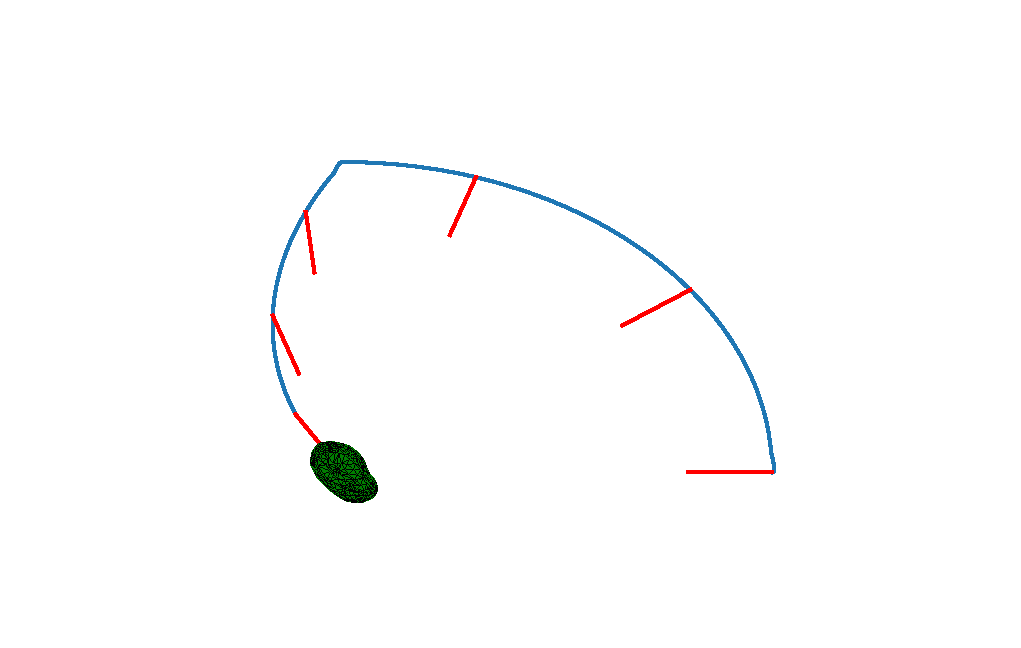
\includegraphics[width=\columnwidth,keepaspectratio,trim={30mm 20mm 30mm 20mm},clip]{figures/traj_fig.pdf}
\end{column}
\end{columns}
\end{frame}

\begin{frame}{Landing Trajectory - Position}
    \begin{itemize}
        \item Transition from horizontal motion to vertical descent
        \begin{itemize}
            \item Move from inertial \( \vb{e}_2 \) to asteroid \( \vb{f}_1 \) axis
            \item Remain in the equatorial plane ( \(\vb{f_1}, \vb{f}_2\) plane)
        \end{itemize}
        \pause
    \item Command is divided into two segments
        \begin{itemize}
            \item Move to \( \vb{f}_1\) along a circular path
            \item Vertical descent along \( \vb{f}_1 \)
        \end{itemize}
    \end{itemize}

    \begin{columns}
        \begin{column}{0.5\textwidth}
            \footnotesize
            \begin{align*}
                \vb{x}_d = 
                \begin{cases}
                    2.550 \begin{bmatrix} \sin{\omega t} & -\cos{\omega t} & 0 \end{bmatrix}, & t \leq t_d \\
                    R_A \begin{bmatrix} \frac{2}{t_d} (t - t_d) + 2.550 & 0 & 0 \end{bmatrix}, & t > t_d , 
                \end{cases}
            \end{align*}
        \end{column}
        \begin{column}{0.5\textwidth}
            \visible<2->{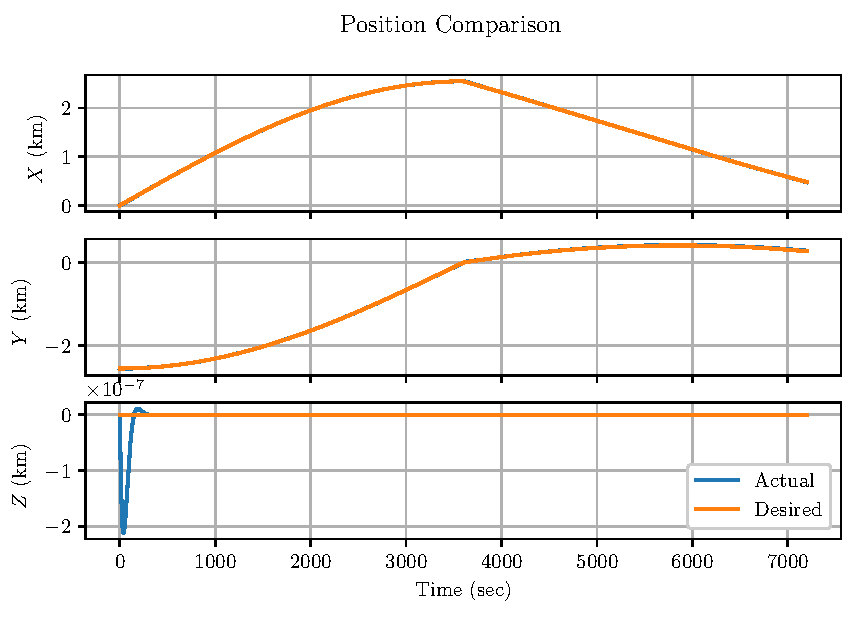
\includegraphics[width=\columnwidth]{figures/pos_fig.pdf}}
    \end{column}
\end{columns}
\end{frame}

\begin{frame}[fragile]{Blender Simulation}
    \only<1>{
    \begin{itemize}
        \item Open-source computer graphics rendering
            \begin{itemize}
                \item Photorealistic Rendering
                \item Realistic material and lighting 
                \item Physics based simulation and game engine
            \end{itemize}
            \pause
        \item Additional capability by utilizing a Python API 
            \begin{itemize}
                \item Load a asteroid shape model
                \item Define camera properties/location
                \item Define light source and position
                \item Render image
            \end{itemize}
\end{itemize}

\begin{center}
    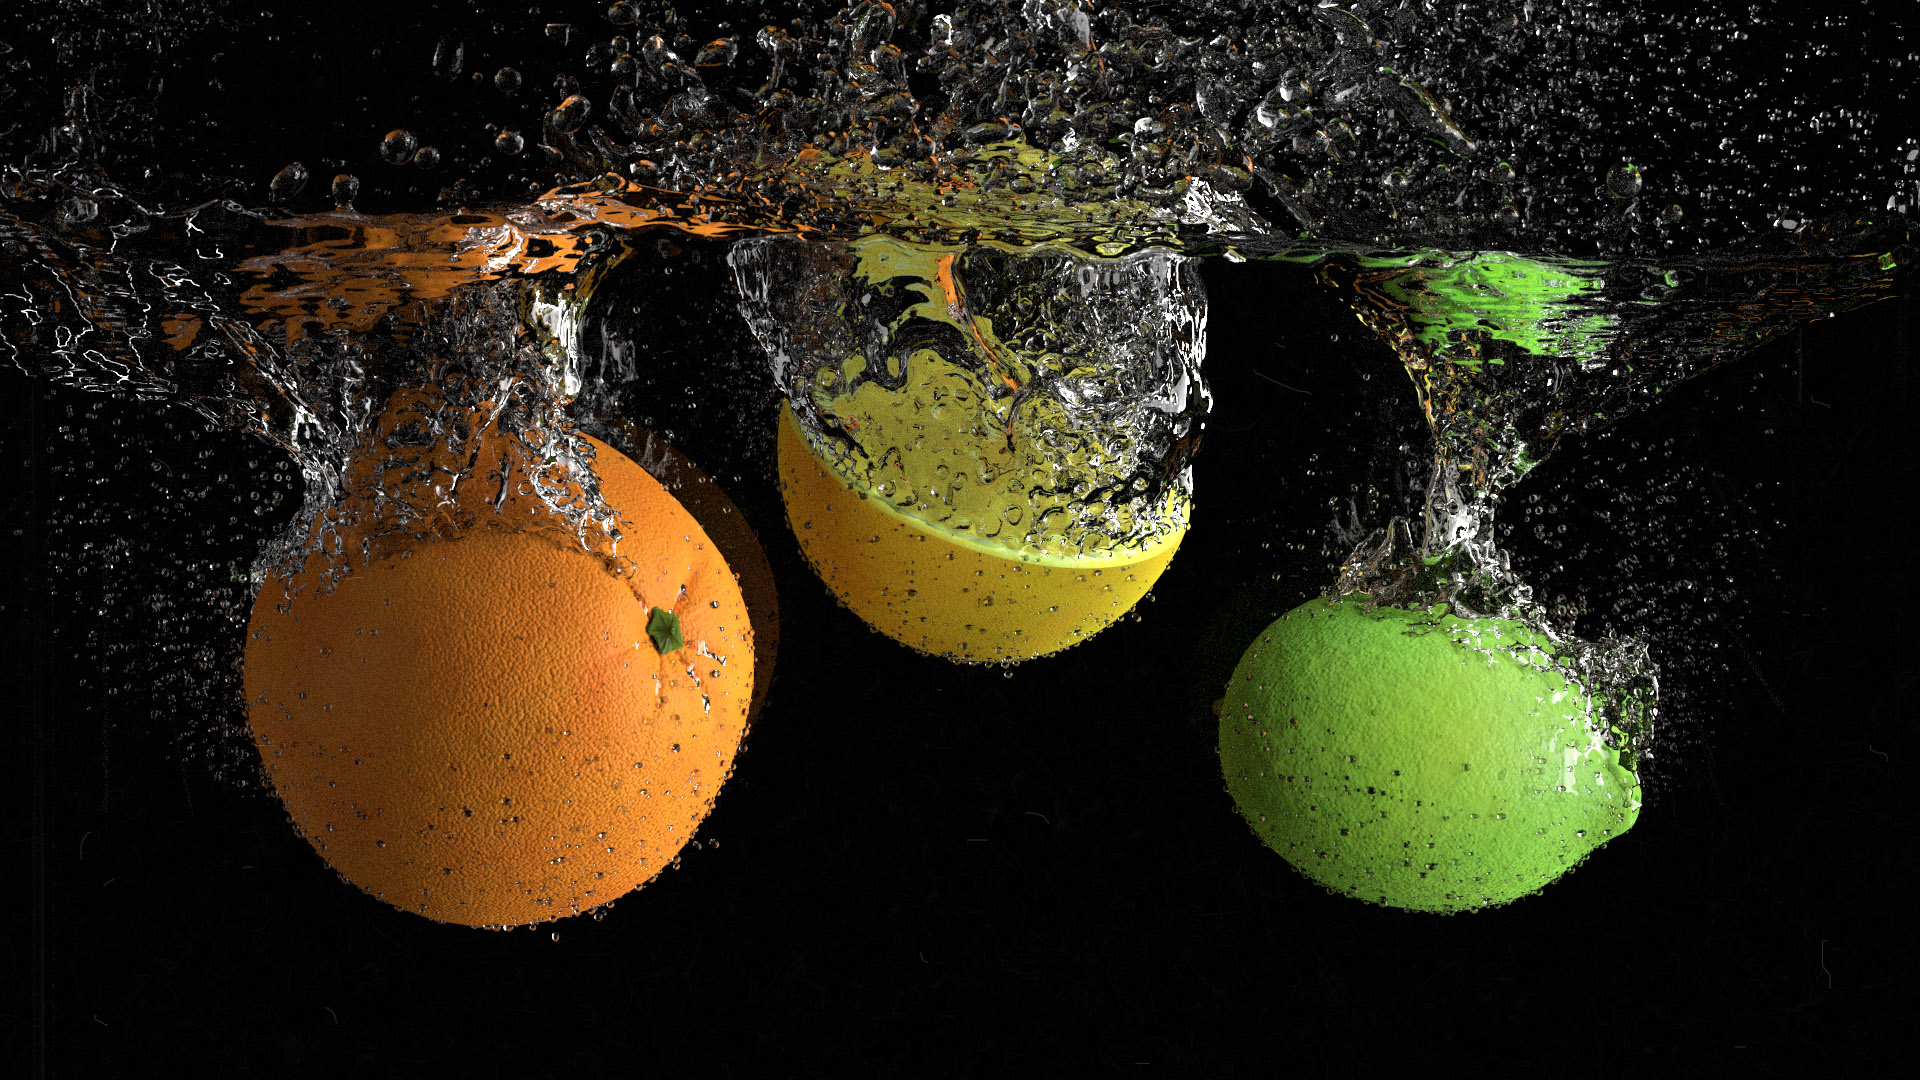
\includegraphics[width=0.5\textwidth,height=0.3\textheight,keepaspectratio]{figures/rendering.jpg}~
    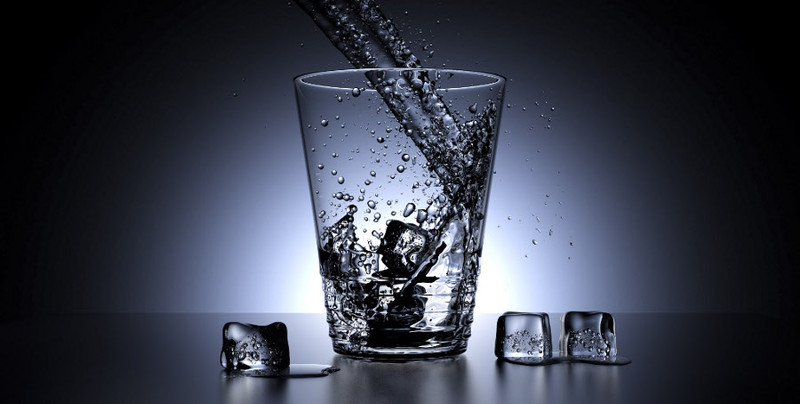
\includegraphics[width=0.5\textwidth,height=0.3\textheight,keepaspectratio]{figures/463e785104.jpg}
\end{center}
}

\only<2>{
    \begin{itemize}
        \item Can render scenes using a graphical interface
    \end{itemize}
    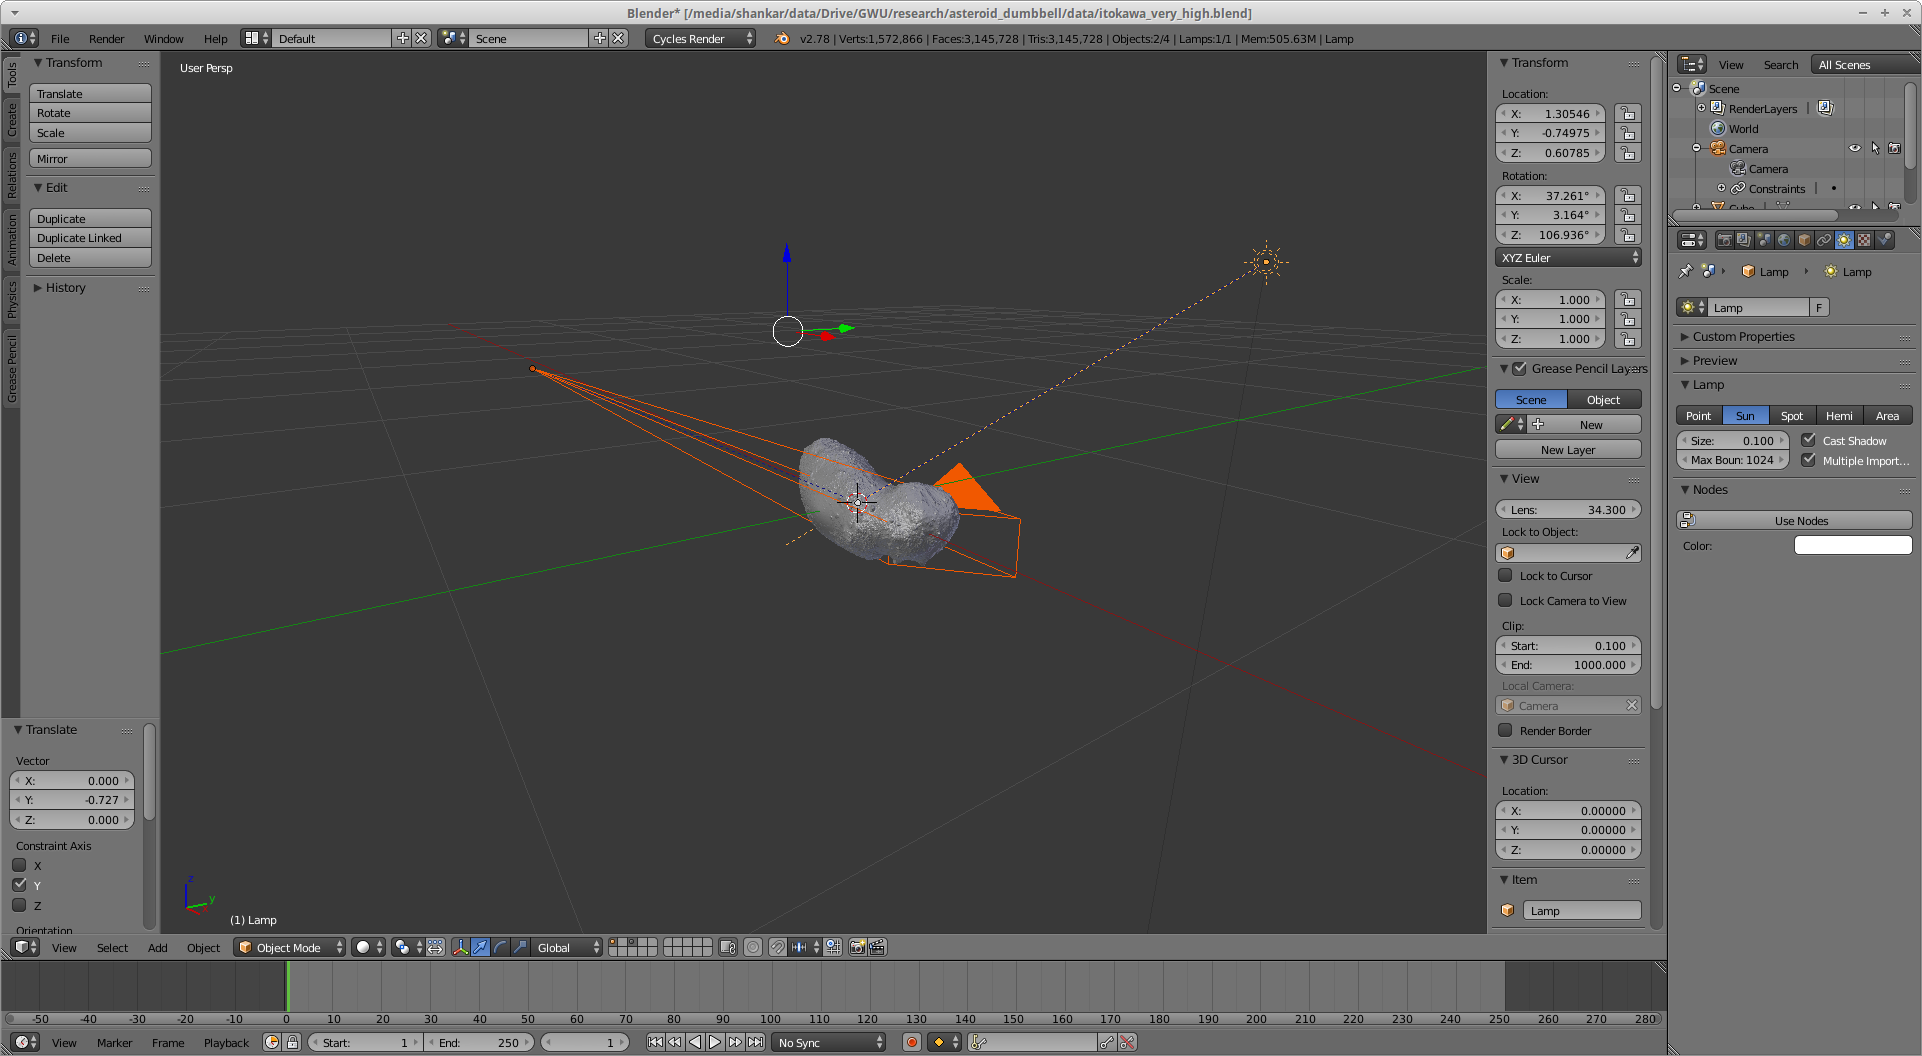
\includegraphics[width=\textwidth]{figures/blender_screenshot.png}
}

\only<3>{
    \begin{itemize}
        \item Python used to generate imagery - incorporate in larger code
    \end{itemize}
    \begin{columns}
        \begin{column}{0.5\textwidth}
        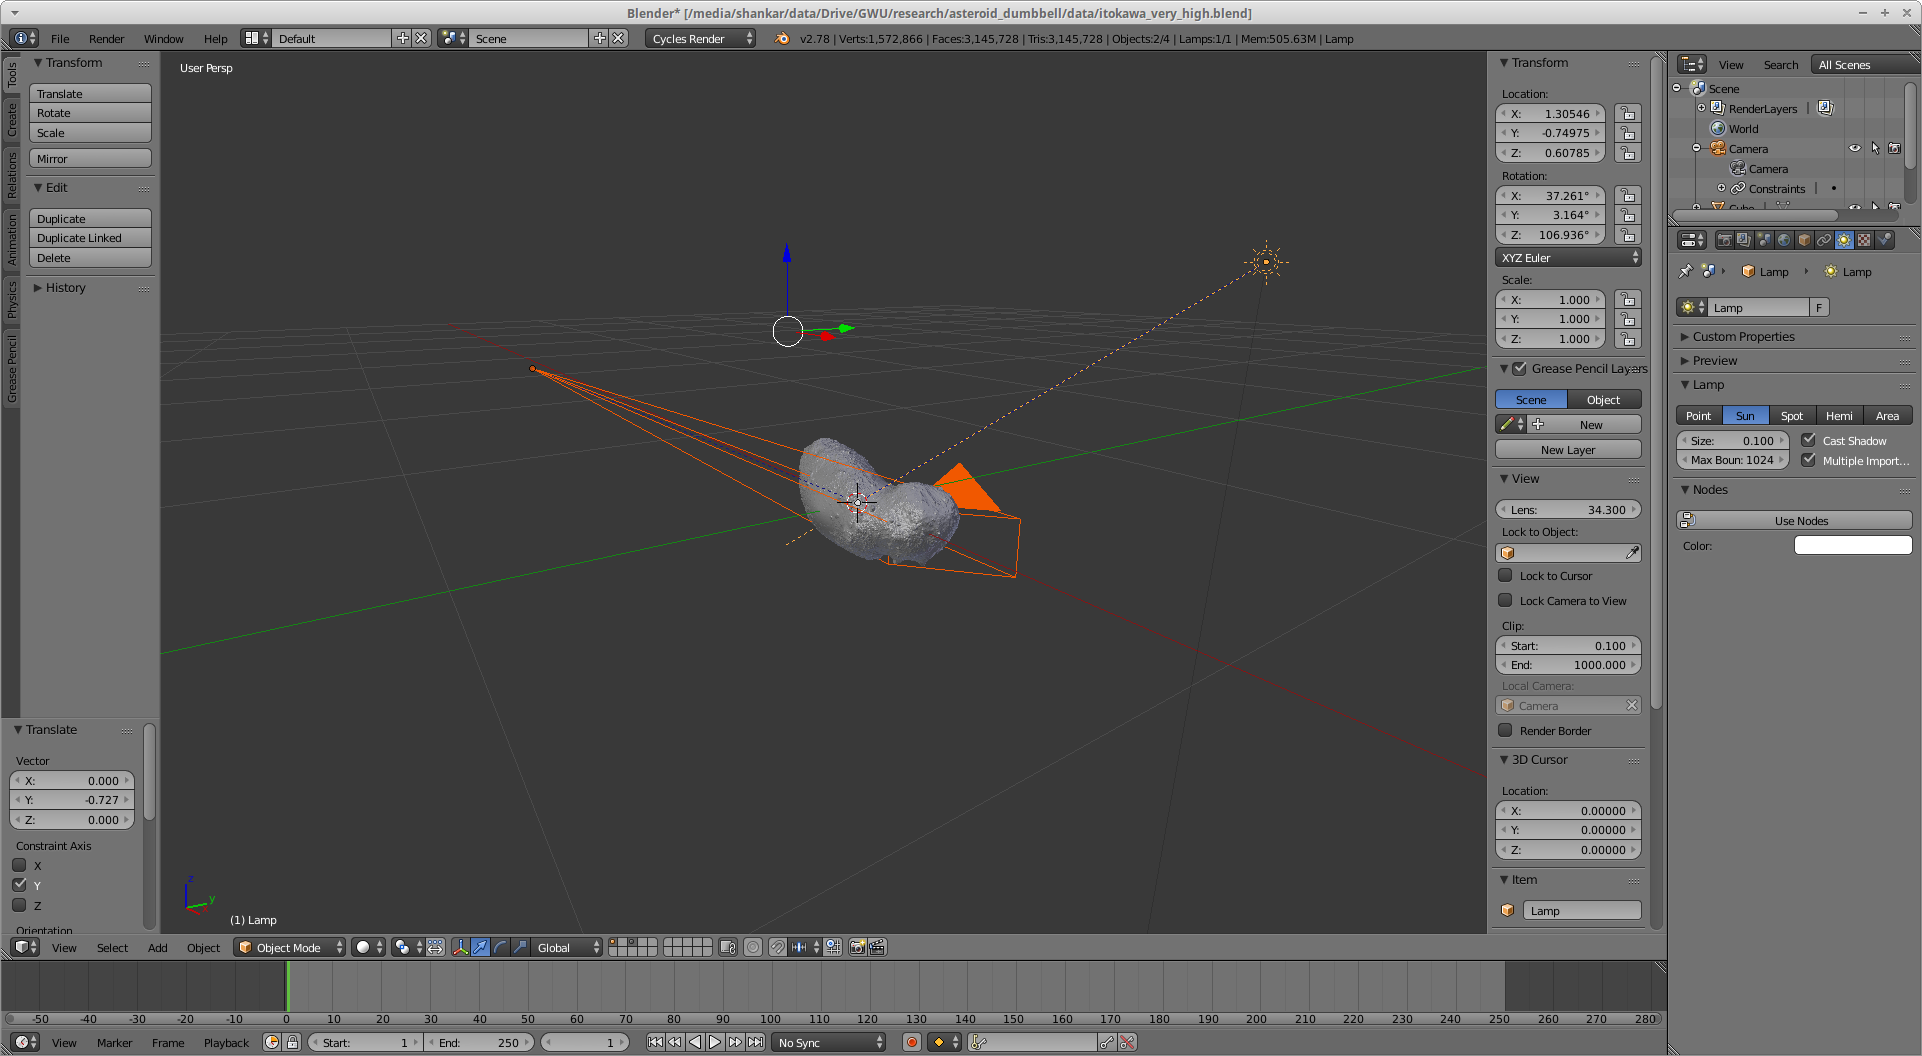
\includegraphics[width=\columnwidth]{figures/blender_screenshot.png}

        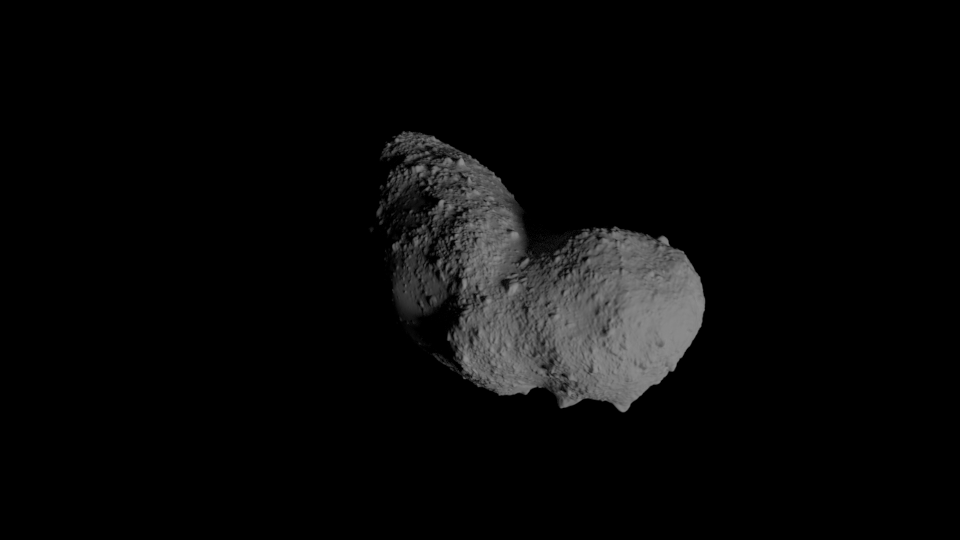
\includegraphics[width=\columnwidth]{figures/itokawa_blender.png}
        \end{column}
        \begin{column}{0.5\textwidth}
            \scriptsize
            \begin{semiverbatim}
            import bpy
    

            scene = bpy.context.scene

            bpy.ops.import\_scene.obj(`ast.obj')

            ast = bpy.data.objects[asteroid]


            ast.scale = [1, 1, 1] 

            ast.location = (0, 0, 0)
          

            scene.render.filepath = `out.png'

            bpy.ops.render.render(write\_still=True)

            \end{semiverbatim}
        \end{column}
    \end{columns}
}
\end{frame}

\begin{frame}{Simulated imagery using Blender}
    \begin{itemize}
        \item Free \& open-source 3D computer graphics program
        \item Offer programmatic interface through Python
        \item Images of Itokawa emulated to match NEAR MSI camera
    \end{itemize}
    \begin{center}
    \movie[loop,showcontrols,externalviewer]{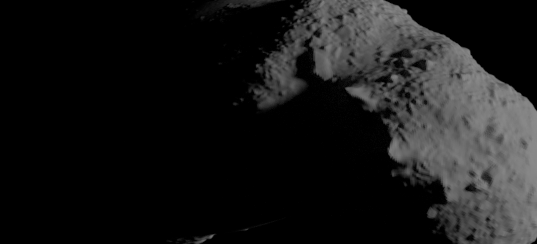
\includegraphics[width=0.5\textwidth]{figures/test000837.png}}{videos/itokawa_landing.mp4}~
    \movie[loop,showcontrols,externalviewer]{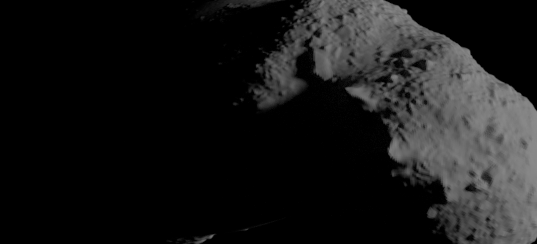
\includegraphics[width=0.5\textwidth]{figures/test000837.png}}{videos/itokawa_high.mp4}
\end{center}
\end{frame}

\begin{frame}{Monocular Localization}
    \begin{itemize}
        \item ORB-SLAM2 - Open-source mapping and localization framework
        \item Allows for real-time monocular based SLAM
        \item Utilized here to demonstrate localization from imagery
    \end{itemize}
    
    \begin{center}
    \movie[loop,showcontrols,externalviewer]{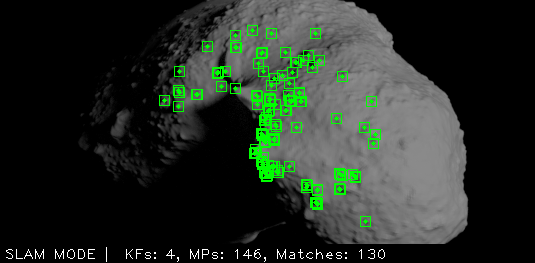
\includegraphics[width=0.5\textwidth]{figures/orbslam_mappoints.png}}{videos/mappoints.mp4}~
    \movie[loop,showcontrols,externalviewer]{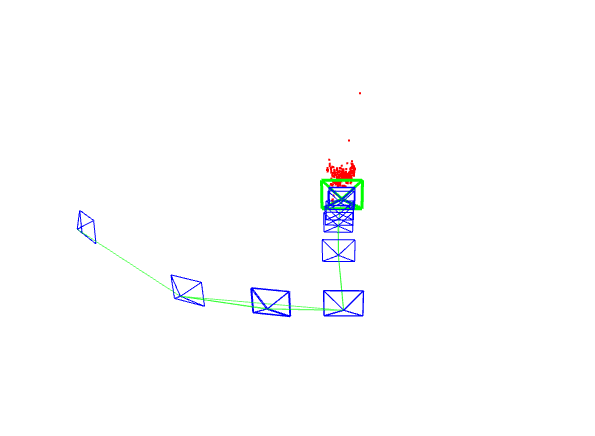
\includegraphics[width=0.5\textwidth]{figures/orbslam_localization.png}}{videos/local_crop.mp4}
\end{center}
\end{frame}
\section*{}
\subsection*{Conclusions}

\begin{frame}{Conclusions}
    \begin{itemize}
        \item Nonlinear controller for landing on an asteroid
        \item Coupled dynamics derived and considered on \SE
        \item Localization performed using simulated monocular imagery
        \item Future Research Goals:
            \begin{itemize}
                \item Utilize state estimates directly in controller
                \item Update shape and gravity model in real-time
            \end{itemize}
    \end{itemize} 
\end{frame}

\begin{frame}[c]{Thank you}
  \centering
  
  \textbf{\large Flight Dynamics \& Control Lab} \\
  Mechanical \& Aerospace Engineering \\
  School of Engineering \& Applied Science
  
  \begin{figure} %figure%
        
\includegraphics[width=0.75\textwidth]{gw_txh_2cs_pos}
    \end{figure}
  
  \url{https://fdcl.seas.gwu.edu}
\end{frame}
\end{document}

